\begin{figure*}[thb!]
  \centering
  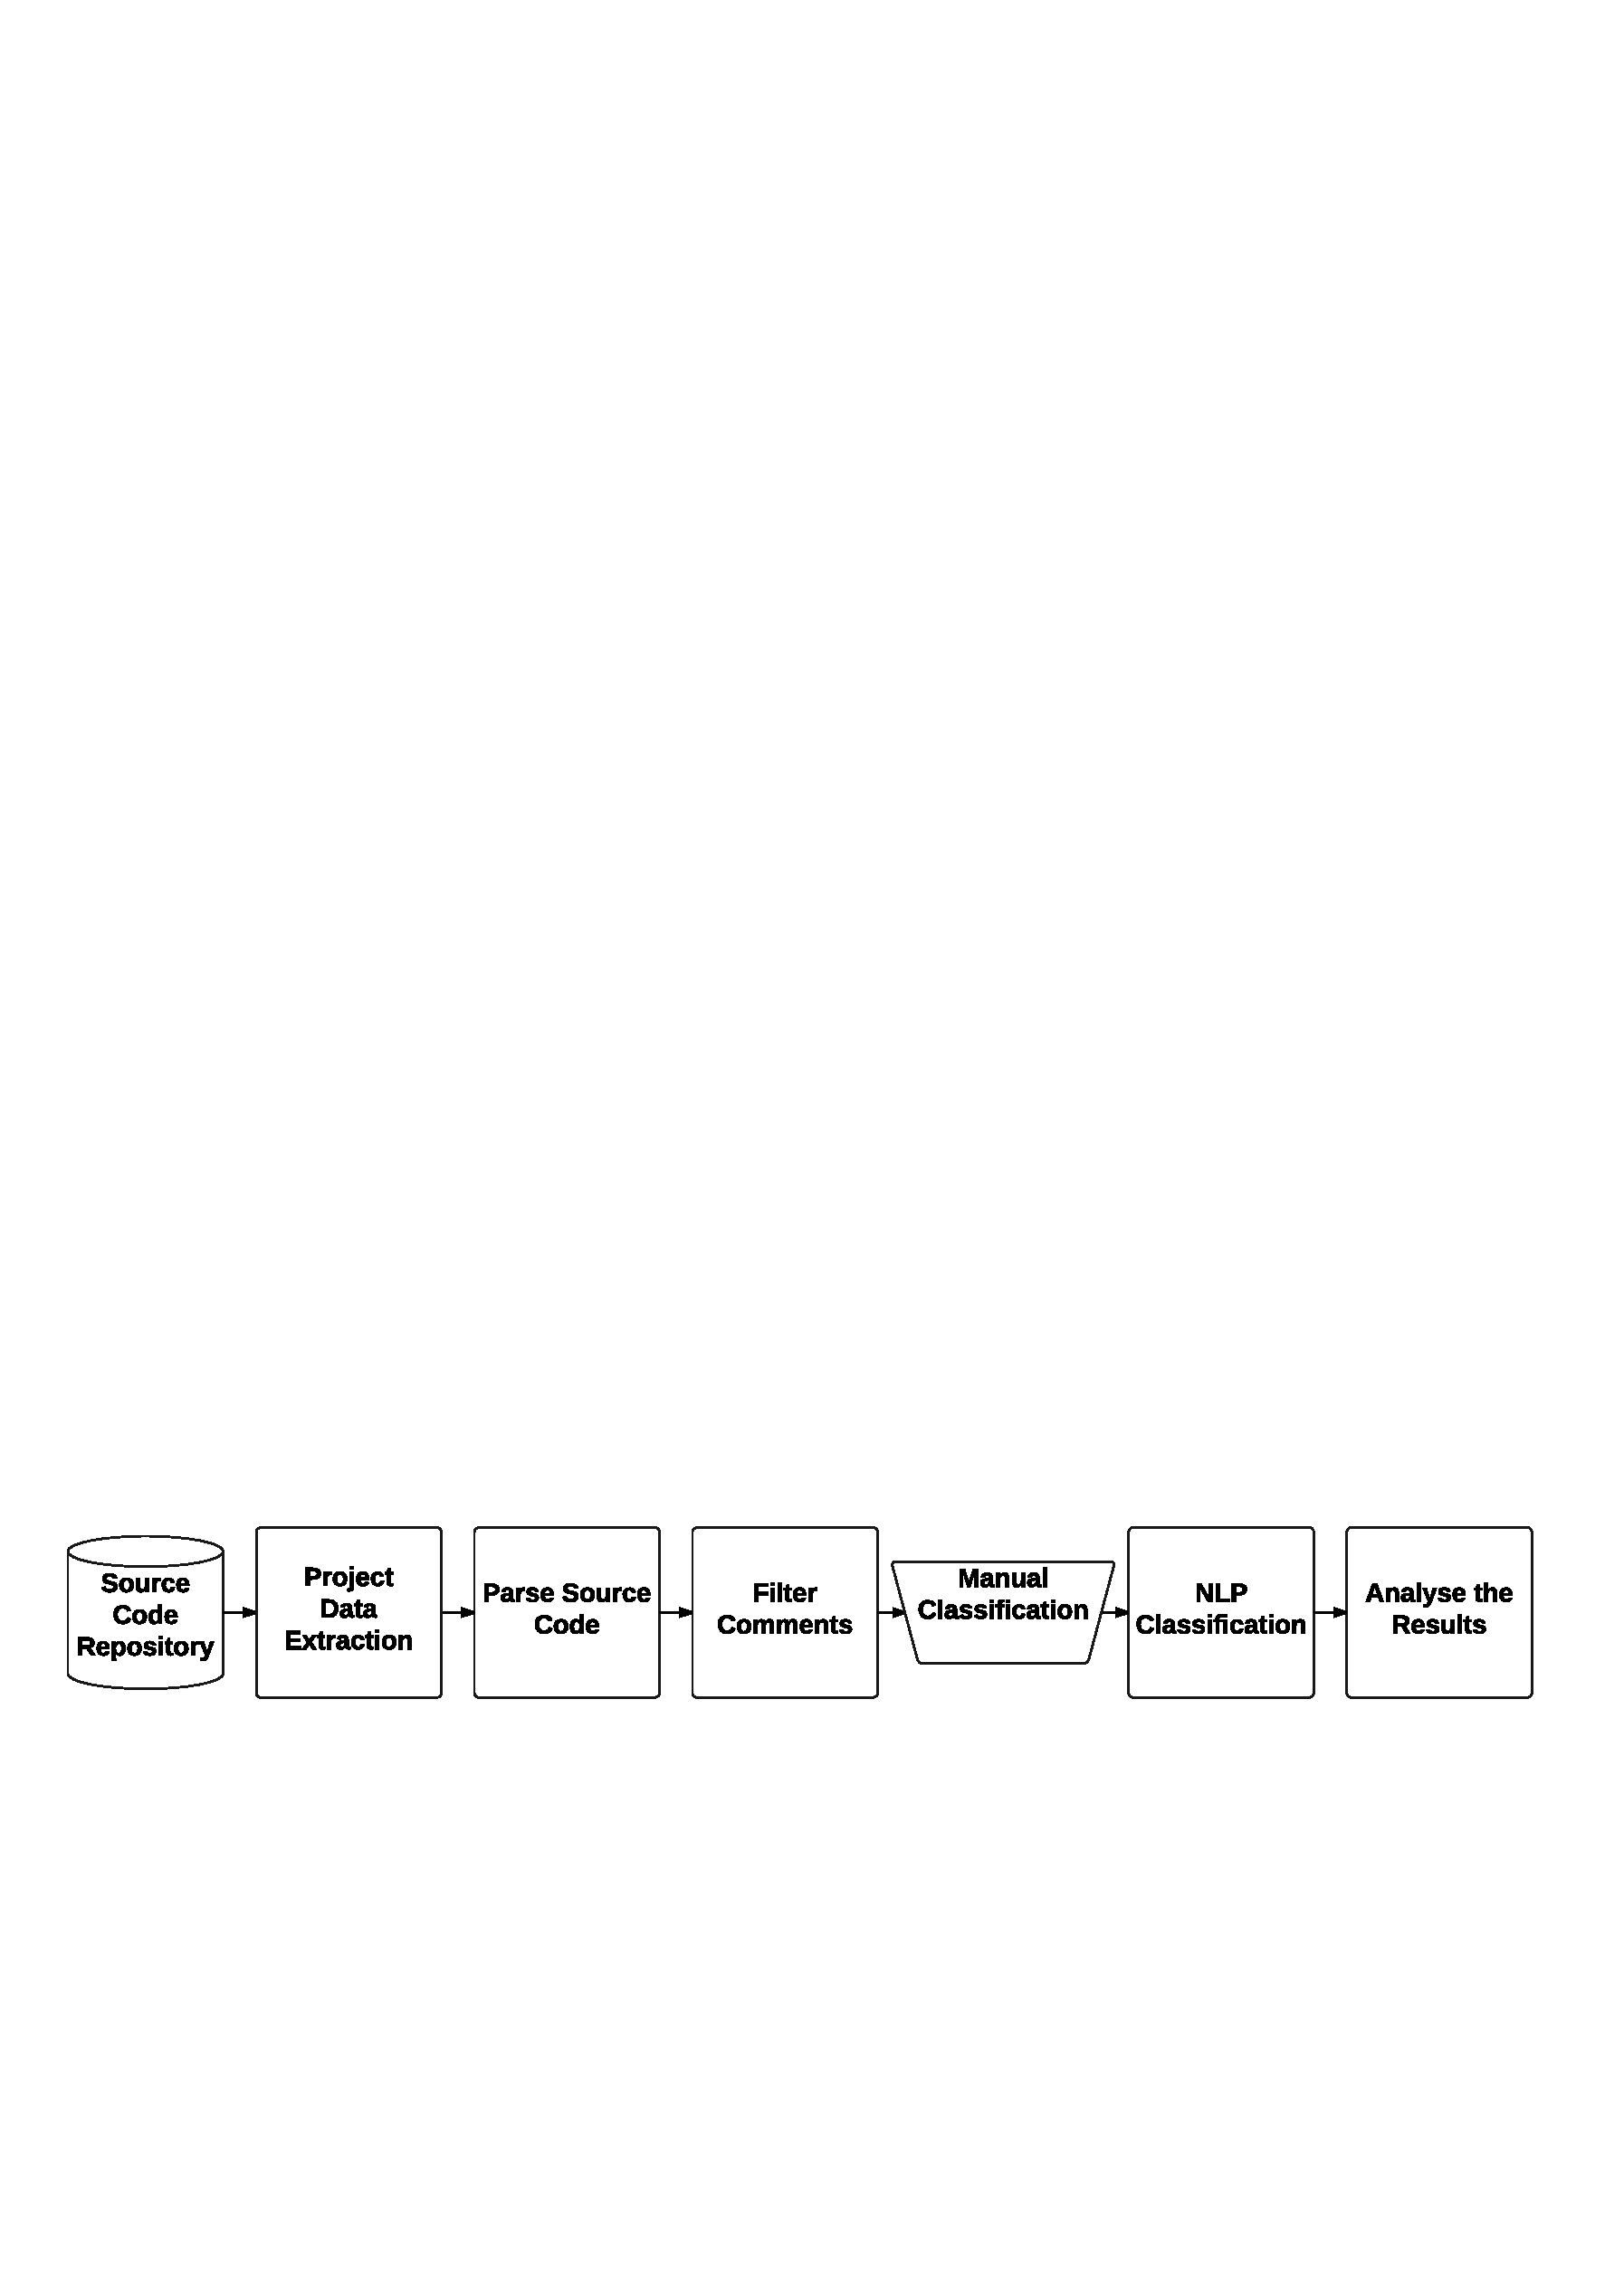
\includegraphics[width=1\textwidth]{approach}
  \caption{Approach overview}
  \label{fig:approach}
\end{figure*}

In a previous work Maldonado and Shihab \cite{MaldonadoMTD2015} shown that between the different types of \SATD the most common types are respectively design technical debt, requirements debt and defect debt. In addition to that  

The main goal of our study is to efficiently identify \SATD as presented in Figure~\ref{fig:approach}. 



The following subsections provides detailed information of each step taken to build our approach.

\subsection{Data Extraction}

To perform our study, we selected ten large open source projects that provides . Due the nature of 

, namely Apache Ant, Apache Jmeter, ArgoUML, Columba, EMF, Hibernate, JEdit, JFreeChart, JRuby and SQuirrel SQL Client. We chose the aforementioned projects, since they belong to different domains, and vary in size (e.g., LOC), and in the number of contributors.

Table~\ref{tab:projDetails} provides statistics about each of the projects used in our study. In total, we obtained more than 258,878 comments, found in 16,249 files. We also include the release used, the number of classes, and the total lines of code (LOC). In our study, we only use the Java files to calculate the LOC. It is important to notice that the number of comments shown for each project does not represent the number of commented lines, but rather the number of individual line, block, and Javadoc comments. 